\section{Réalisation du logiciel}

Maintenant que nous avons vu les outils utilisés pour réaliser simulationRainOfMusic, nous allons présenter son architecture et les éléments importants de son implémentation.

\subsection{Architecture}
Dans les premières étapes de la réalisation du logiciel, nous avons établi l'architecture en respectant certains points qui nous paraissaient essentiels à notre projet.

Tout d'abord, notre logiciel étant un logiciel de visualisation avant tout, il nous semblait plus clair de choisir une architecture modèle-vue. Cela nous permettait d'avoir une séparation nette entre la partie données des robots et la partie modélisation et affichage 3D. 

Ensuite, le projet contenant des robots Metabot mais aussi des drones, il nous avait été demandé à ce que notre logiciel soit modulaire, facilitant ainsi l'ajout de nouvaux types de robots. C'est pour cela que nous avons choisi dans notre implémentation d'utiliser le mécanisme en C++ des \verb|template| pour assurer ce côté modulaire.

Enfin, une attention particulière a été portée à la classe \verb|Parameter|, jouant le rôle d'intermédiaire entre i-score et l'interface utilisateur de notre logiciel. Cette classe occupe une place importante dans le projet puisqu'elle permet de mettre à jour les valeurs en fonction des modifications apportées à notre interface et à i-score.

Par ailleurs, l'intégration de la classe \verb|Parameter| dans l'architecture s'est déroulée naturellement : elle prend le rôle du contrôleur qui met à jour les valeurs du modèle en fonction des données modifiées sur la vue qui est aussi l'interface utilisateur.

		
\subsection{Implémentation}

Dans cette partie, nous allons présenter simulationRainOfMusic en s'intéressant d'un peu plus près au code qui permet de remplir les trois objectifs principaux: la visualisation, la communication et la simulation.

\subsubsection{Visualisation}

La mise en place de la scène 3D a été réalisée assez facilement grâce à la caméra de la classe \verb|EasyCam| déjà implémentée dans openFrameworks. Ainsi l'utilisateur a la possibilité de se déplacer et de zoomer dans la scène 3D grâce à la souris. Les robots peuvent être représentés par des modèles 3D importés par l'utilisateur. Si aucun modèle n'est trouvé ou importé, le logiciel utilisera un cube à la place. Durant la réalisation du projet, nous avons choisi d'utiliser des modèles 3D d'araignées visibles dans la figure \ref{interface} pour représenter les metabots quadrupèdes.

\begin{figure}[H]
\centering
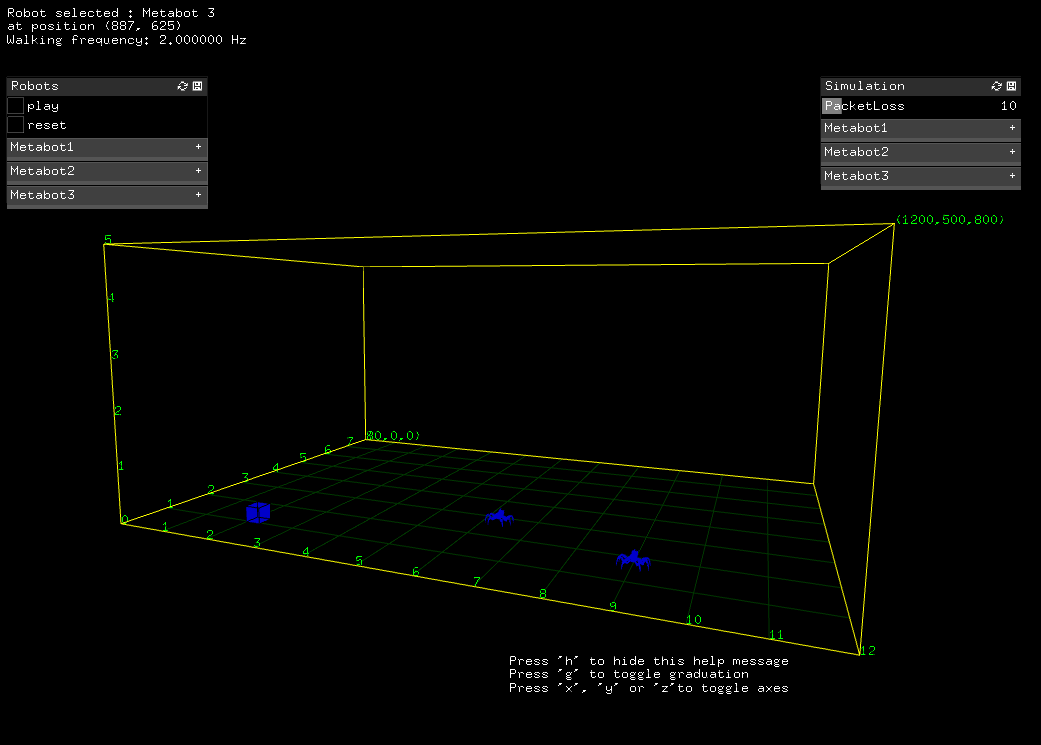
\includegraphics[scale=0.37]{imgs/view2}
\caption{Vue générale de l'interface graphique}
\label{interface}
\end{figure}

L'utilisateur peut également sélectionner un robot. Lorsqu'un robot est sélectionné, différentes caractéristiques le concernant s'affichent en haut à gauche de la fenêtre de simulation (le message est représenté en figure \ref{mselec}). Ces caractéristiques sont composées d'un identifiant, du type de robot (metabot ou drone) et de la position. La sélection se fait grâce à la détection de la couleur unique au robot.

\begin{figure}[H]
\centering
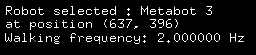
\includegraphics[scale=0.7]{imgs/selection}
\caption{Message de sélection d'un robot}
\label{mselec}
\end{figure}

Si deux robots risquent de rentrer en collision, ceux-ci sont entourés d'un cercle rouge (figure \ref{col}) pour alerter l'utilisateur et un message informatif indiquant la position et le robot entré en collision est affiché (figure \ref{mcol}).

\begin{figure}[htbp]
\begin{minipage}[c]{.45\linewidth}
\begin{center}
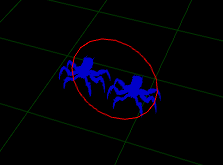
\includegraphics[scale=0.45]{imgs/collision}
\caption{Exemple d'avertissement de collision}
\label{col}
\end{center}
\end{minipage}
\hspace*{0.5cm}
\begin{minipage}[c]{.5\linewidth}
\begin{center}
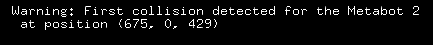
\includegraphics[scale=0.6]{imgs/mcollision}
\caption{Message contenant des informations sur la collision}
\label{mcol}
\end{center}
\end{minipage}
\end{figure}

En plus de ces informations, un panel (figure \ref{pan})permet de visualiser et de modifier les positions et vitesses des robots via des sliders. Un emplacement dans l'onglet affiche également si les robots sont en collision ou non. Une fois des vitesses choisies, un bouton play permet de voir la chorégraphie. 

\begin{figure}[H]
\centering
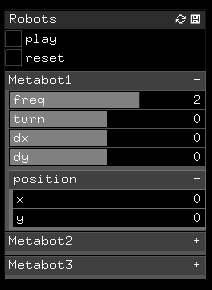
\includegraphics[scale=0.6]{imgs/panel2}
\caption{Panel de visualisation}
\label{pan}
\end{figure}

Enfin l'utilisateur a la possibilité de rajouter des axes selon x, y et z en plus pour mieux situer les robot dans l'espace en plus des axes principaux. Ceux-ci sont gradués au mètre, comme on peut le voir sur la figure \ref{grad} suivante :
					
\begin{figure}[H]
\centering
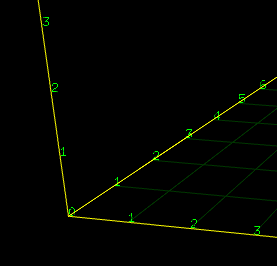
\includegraphics[scale=0.8]{imgs/graduation}
\caption{Graduation des axes}
\label{grad}
\end{figure}

\subsubsection{Communication}

La communication avec i-score est possible grâce à l'API d'OSSIA et à la classe \verb|Network|. Cette dernière permet d'initier la communication avec i-score. A la construction d'un objet Network, une fonction sur un thread qui fait la publication s'éxécute : elle déclare le programme comme un objet réseau, que l'on peut ajouter dans i-score en lui donnant son nom et le numéro de port associé, et qui constitue la racine de l'arbre du réseau. Elle envoie ensuite sur le réseau le noeud 'scène' en le déclarant comme noeud fils du programme.

A l'instanciation d'un robot, celui-ci est ajouté à l'arbre du réseau comme fils du noeud 'scène'. Chacun de ses attributs est aussi publié. Lorsqu'un attribut dans l'arbre publié sur le réseau est modifié via l'interface utilisateur d'i-score, sa valeur est mise à jour dans simulationRainOfMusic grâce à une fonction (\verb|Callback|). Cet arbre est visible sur i-score comme présenté dans la figure \ref{tr}.

\begin{figure}[H]
\centering
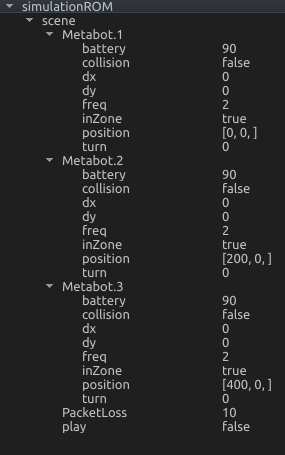
\includegraphics[scale=0.7]{imgs/tree}
\caption{Exemple d'arbre visible sur i-score}
\label{tr}
\end{figure}

La racine de l'arbre est notre logiciel simulationRainOfMusic. Elle a un fils nommé 'scene', qui a lui-même comme fils l'ensemble des robots.

Pour ajouter la communication entre simulationRainOfMusic et son interface, la classe \verb|Parameter| a été créée. Elle encapsule la classe \verb|ofParameter| de openFrameworks. La classe \verb|ofParameter| permet de lier un listener à une valeur affichée sur l'interface. Le listener est une fonctionnalité qui permet d'être constamment à l'écoute de toute modification opérée au niveau de l'interface. Par exemple, un objet de la classe \verb|ofParameter| peut être utilisé pour lier une valeur position en x avec un slider dans l'interface utilisateur : le fait de bouger le slider va mettre à jour la valeur représentant la position en x. De cette façon, utiliser une variable de type \verb|ofParameter| permet de lier un attribut de robot à l'interface utilisateur. 

Ainsi, la classe \verb|Parameter| encapsulant \verb|ofParameter| utilise un listener \verb|Callback| vers i-score et un listener vers l'interface de simulationRainOfMusic. Pour voir plus précisément ce qui se passe dans les deux sens, voici deux diagrammes de séquence sur les figures \ref{diag1} et \ref{diag2} :

\begin{figure}[H]
\begin{center}
\includegraphics[scale=0.6]{i-scoretogui}
\caption{Modification sur i-score et mise à jour du GUI}
\label{diag1}
\end{center}
\end{figure}

Lorsqu'une valeur est modifiée sur i-score, l'arbre partagé est automatiquement mis à jour. Le paramètre correspondant dans simulationRainOfMusic ayant un \verb|Callback|, ce changement est automatiquement détecté. La valeur du paramètre dans simulationRainOfMusic est alors mise à jour et la fonction \verb|set| est appelée pour mettre à jour la valeur sur l'interface (GUI).

\begin{figure}[H]
\begin{center}
\includegraphics[scale=0.6]{guitoi-score}
\caption{Modification du GUI et mise à jour d'i-score}
\label{diag2}
\end{center}
\end{figure}

Quand une valeur est modifiée sur le GUI, listener correspondant à ce paramètre détecte la modification. On vérifie alors que la valeur correspondant sur l'arbre partagé doit bien être changée. Si c'est le cas, on la met à jour sur l'arbre partagé et la valeur sur i-score se met automatiquement à jour grâce à son \verb|Callback|. 

\subsubsection{Simulation}

Concernant la simulation, un des aspects le plus important et étroitement relié à la visualisation est l'échelle spatio-temporelle des mouvements des Metabots. En effet, d'après la documentation technique de ces robots \footnote{\url{https://github.com/Rhoban/Metabot/blob/master/docs/}}, les commandes de mouvements envoyées au robot sont en millimètre par seconde. Ainsi, dans notre logiciel, les vitesses envoyées à travers l'interface utilisateur sont en millimètre par seconde. Cela permet aux utilisateurs d'avoir une simulation de la chorégraphie proche de la réalité.

Ensuite, nous avons implémenté trois évènements qui peuvent arriver au cours de la chorégraphie et qui nous semblaient utiles à mettre en place pour l'artiste simulant la chorégraphie. 

Le premier est la panne du robot dûe à un niveau de batterie nul. Pour cela, un modèle simple linéaire en fonction de la distance parcourue a été implémenté. Néanmoins, ce modèle pourrait être modifié pour obtenir une modélisation plus fidèle à la consommation réelle des batteries des metabots. Le niveau de consommation des différents metabots est visible dans le panel simulation de l'interface graphique. 

Le deuxième évènement est la perte de paquets lors de la communication entre les robots et le logiciel i-score envoyant les commandes. Identiquement, au point précédent, un modèle simple a été implémenté dû fait que cette communication n'est pas encore établié dans l'état actuel du projet. Une probabilité de perte de paquets a été introduite dans notre implémentation, et permet de simuler les pertes de paquets lorsque notre simulation reçoit de i-score les modifications apportées aux données de l'arbre partagé. 

Lorsqu'un paquet est perdu, le metabot ne verra donc pas ses paramètres changées et gardera les précédentes. Concrètement, lors d'une chorégraphie cela signifierait que les metabots pourraient garder leur vitesse précédente et ne s'arrêterait pas. Ce comportement est fidèle à la réalité, puisque les metabots gardent leurs paramètres tant qu'ils ne reçoivent pas de commandes les modifiant. 

Une fois que le protocole de communication entre les robots et i-score sera en place, des tests pourraient être conduits et permettront d'obtenir une idée approximative du pourcentage de perte de paquets, celle-ci pourra être reflétée dans notre logiciel de simulation.

Le panel de simulation est montré dans la figure \ref{spa} suivante :

\begin{figure}[H]
\centering
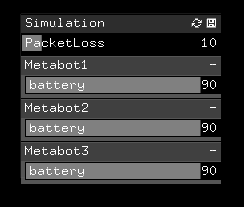
\includegraphics[scale=1]{imgs/spanel}
\caption{Panel de simulation}
\label{spa}
\end{figure} 

Le troisième évènement qui pourrait arriver peut être le plus fréquemment lors d'une simulation réelle de la chorégraphie avec les robots est la possibilité de collision entre les différents robots. Pour cela, une première approche "manuelle" a été implémentée qui se basait sur un système simple vérifiant la taille des robots et leur position. Par la suite, la possibilité d'utiliser des bibliothèques de moteur physique a été étudiée mais n'a pas aboutie. La raison principale à cela a été que ces bibliothèques (ofxBullet, ofxMSAPhysics) ne pouvaient être compilées suite à des erreurs dans le code publié sur GitHub. Il est fort probable que ce problème était dû à des commits récents mais nous n'avons pas insisté dans la suite du projet pour recompiler ces bibliothèques. 

